\documentclass{article}
\usepackage[utf8]{inputenc}

\title{Final Project - Capillary Rise}
\author{Osamu Katagiri-Tanaka : A01212611}
\date{November 25, 2020} %\date{\today}

% import math symbols
\usepackage{amsmath, esint}
\usepackage{cancel}

% multiline equations
\usepackage{breqn}

% import code snippets
\usepackage{listings}
\usepackage{xcolor}
\definecolor{codegreen}{rgb}{0,0.6,0}
\definecolor{codegray}{rgb}{0.5,0.5,0.5}
\definecolor{codepurple}{rgb}{0.58,0,0.82}
\definecolor{backcolour}{rgb}{0.99,0.99,0.96}
\lstdefinestyle{mystyle}{
  backgroundcolor   = \color{backcolour},
  commentstyle      = \color{codegreen},
  keywordstyle      = \color{magenta},
  numberstyle       = \tiny\color{codegray},
  stringstyle       = \color{codepurple},
  basicstyle        = \ttfamily\small,
  breakatwhitespace = false,
  breaklines        = true,
  captionpos        = b,
  keepspaces        = true,
  numbers           = left,
  numbersep         = 2pt,
  showspaces        = false,
  showstringspaces  = false,
  showtabs          = false,
  tabsize           = 2,
  aboveskip         = 0.1em,
  belowskip         = 0.1em
}
\lstset{style=mystyle}

% import hyperlinks
\usepackage{hyperref}
\hypersetup{
  colorlinks = true,
  linkcolor  = red,
  filecolor  = red,
  citecolor  = red,
  urlcolor   = red
}

% import continuous lists
\usepackage{enumitem}

% format margins and paper size
\usepackage{geometry}
\geometry{
	paper         = a4paper, % Change to letterpaper for US letter
	inner         = 2.5cm,   % Inner margin
	outer         = 2.5cm,   % Outer margin
	bindingoffset = 0.5cm,   % Binding offset
	top           = 1.5cm,   % Top margin
	bottom        = 1.5cm    % Bottom margin
}

% import figure handler
\usepackage{graphicx}

% import references handler
\usepackage[
  style     = ieee,         % references format style
  backend   = biber,        % choose the processing program
  natbib    = true,         % enable additional reference formats
  citestyle = numeric-comp, % enable multiple citations
  sortcites = true,         % sort references in multiple citations
  sorting   = nyt           % sort the reference table
]{biblatex}
\addbibresource{references.bib}

% Note that ‘d’ in the differential is conventionally set in roman.
\newcommand{\ud}{\,\mathrm{d}}

% Paragraph spacing
\setlength{\parskip}{0.2cm}           % spacing between paragraphs
\renewcommand{\baselinestretch}{1.25} % spacing between lines

\begin{document}

\maketitle

%\subsection*{Simulate the cooling of apple/avocado considering, convection and radiation.}

Capillary rise is a phenomenon depicted when a small glass capillary tube is introduced into a liquid reservoir and the liquid rises within the tube. The rise is caused by a combination of adsorption and capillarity. \cite{Zhmud2000} The gas-liquid interface to becomes curved as the liquid moves onto the surface of the tube. This effect is the result of a difference in pressures, since the pressure in the liquid is less than the gas pressure. The difference in pressure causes the liquid to rise above the reservoir level to reach hydrostatic conditions. \cite{Zhmud2000} It is known that the height to which a fluid rises within a capillary is inversely proportional to the tube's inner diameter. In this study, ANSYS Fluent was used to report the fluid height within a capillary tube. \cite{Zhmud2000}

\begin{figure}[h!]
	\centering
	
\includegraphics[scale=0.5]{./schematic.png}
	\caption{Schematic of capillary rise}
	\label{img:schematic}
\end{figure}

A 2-dimensional schematic of the capillary rise is shown in Figure \ref{img:schematic}. The capillary tube is simulated by two parallel lines with a spacing $w$ of $0.5 \textrm{mm}$, summerged in a water reservoir. The submerged section of the capillary tube $h_o$ is $5 \textrm{mm}$. The initial height of water $h_l$ in the reservoir is set at $5 \textrm{mm}$. The remaining space is simulated as air at atmospheric pressure. An Eulerian 2-phase system is configured within Fluent to enable the liquid rise due to adhesion, inertia, gravity, and viscous forces. The following assumptions were made: a) the liquid level of the reservoir are negligible compared to that in the capillary as the free surface in the reservoir is much larger; and b) Air and water are in-compressible and of constant viscosity with properties depicted in Table \ref{tab:materials}

\begin{table}[h!]
\centering
\begin{tabular}{ccc} 
 \hline
 property & air & water \\
 \hline
 density $\rho \textrm{ [kg} / \textrm{m}^3 \textrm{]}$ & $1.225$                & $998.2$ \\ 
 surface tension $\sigma \textrm{ [N} / \textrm{m]}$    & $-$                    & $0.072$ \\
 viscosity $\eta \textrm{ [Pa} \cdot \textrm{s]}$       & $0.179 \times 10^{-6}$ & $1.003 \times 10^{-3}$ \\
 \hline
\end{tabular}
\caption{Table to test captions and labels}
\label{tab:materials}
\end{table}

\begin{figure}[h!]
	\centering
	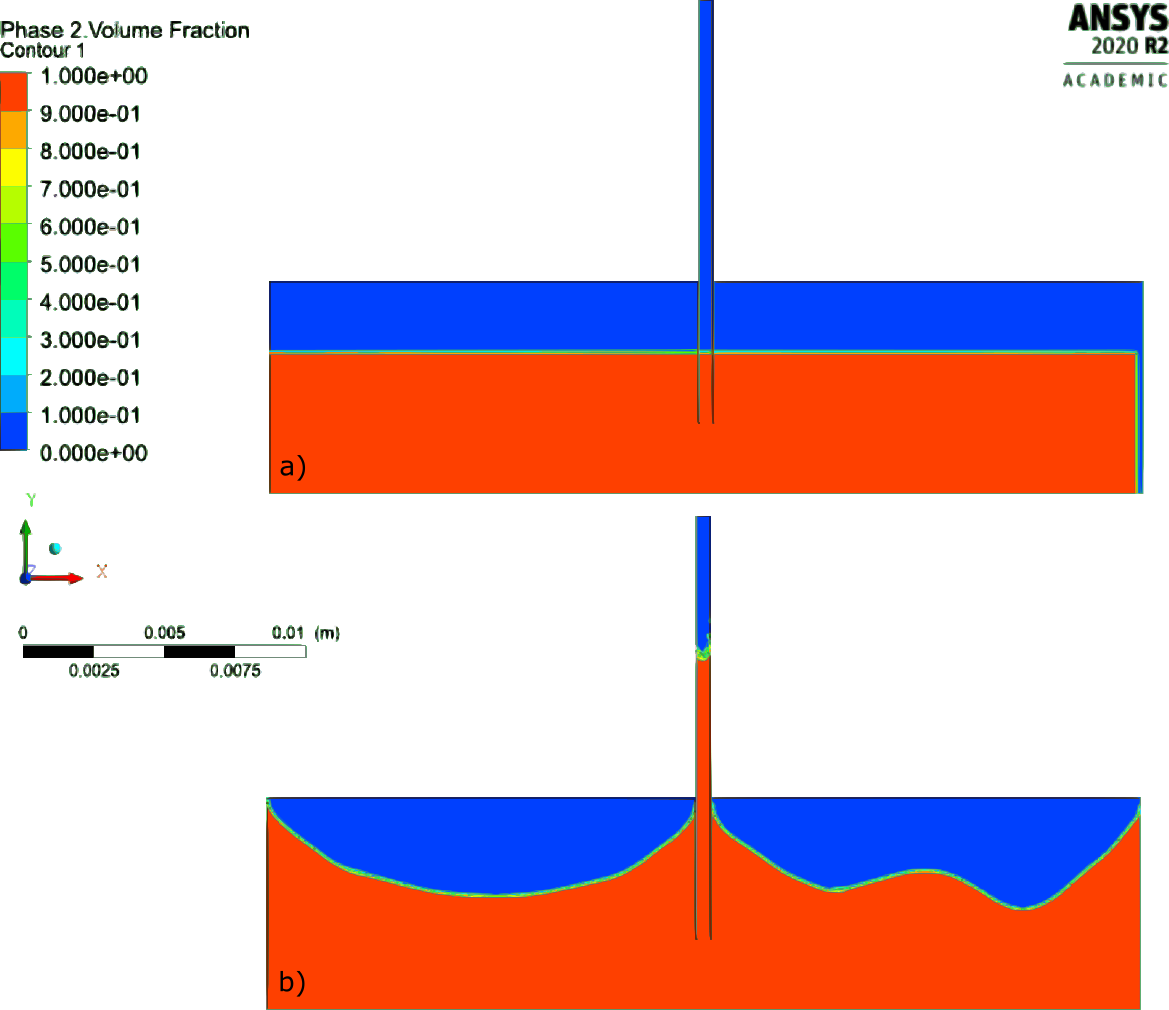
\includegraphics[width=1.00\textwidth]{./SimStoE.png}
	\caption{CFD simulation results. Phase 2 represents water. a) Initial conditions b) hydrostatic/stable conditions}
	\label{img:CFDresults}
\end{figure}

Figure \ref{img:CFDresults} depicts the actual dimensions, the initial and stable conditions of both phases. As depicted in the Figure \ref{img:modelVScfd}, the fluid height $h(t)$ increases with time. The simulation results match with Lucas–Washburn equation which describes the capillary height to be proportional to the square-root of time. \cite{Fisher1980, Oliva1975}. The Lucas–Washburn model considers a quasi-steady state in which the capillary force is balanced against the gravity and viscous forces. \cite{Zhmud2000} as follows:

\begin{dmath}
\frac{d z}{d t} = \frac{\gamma r cos \theta}{4 \eta z} - \frac{r^2 \rho g}{8 \eta}
\end{dmath}

The predictions of Lucas–Washburn's equation agree with the ANSYS simulation results. It is noticeable that at $t_{\infty}$, the height stabilize at $6 \textrm{mm}$ and the quasi-steady state assumption becomes more relevant. CFD was used to simulate the capillary rise of water in a tube. The the results obtained using CFD and Lucas–Washburn model showed good agreement.

 \begin{figure}[h!]
	\centering
	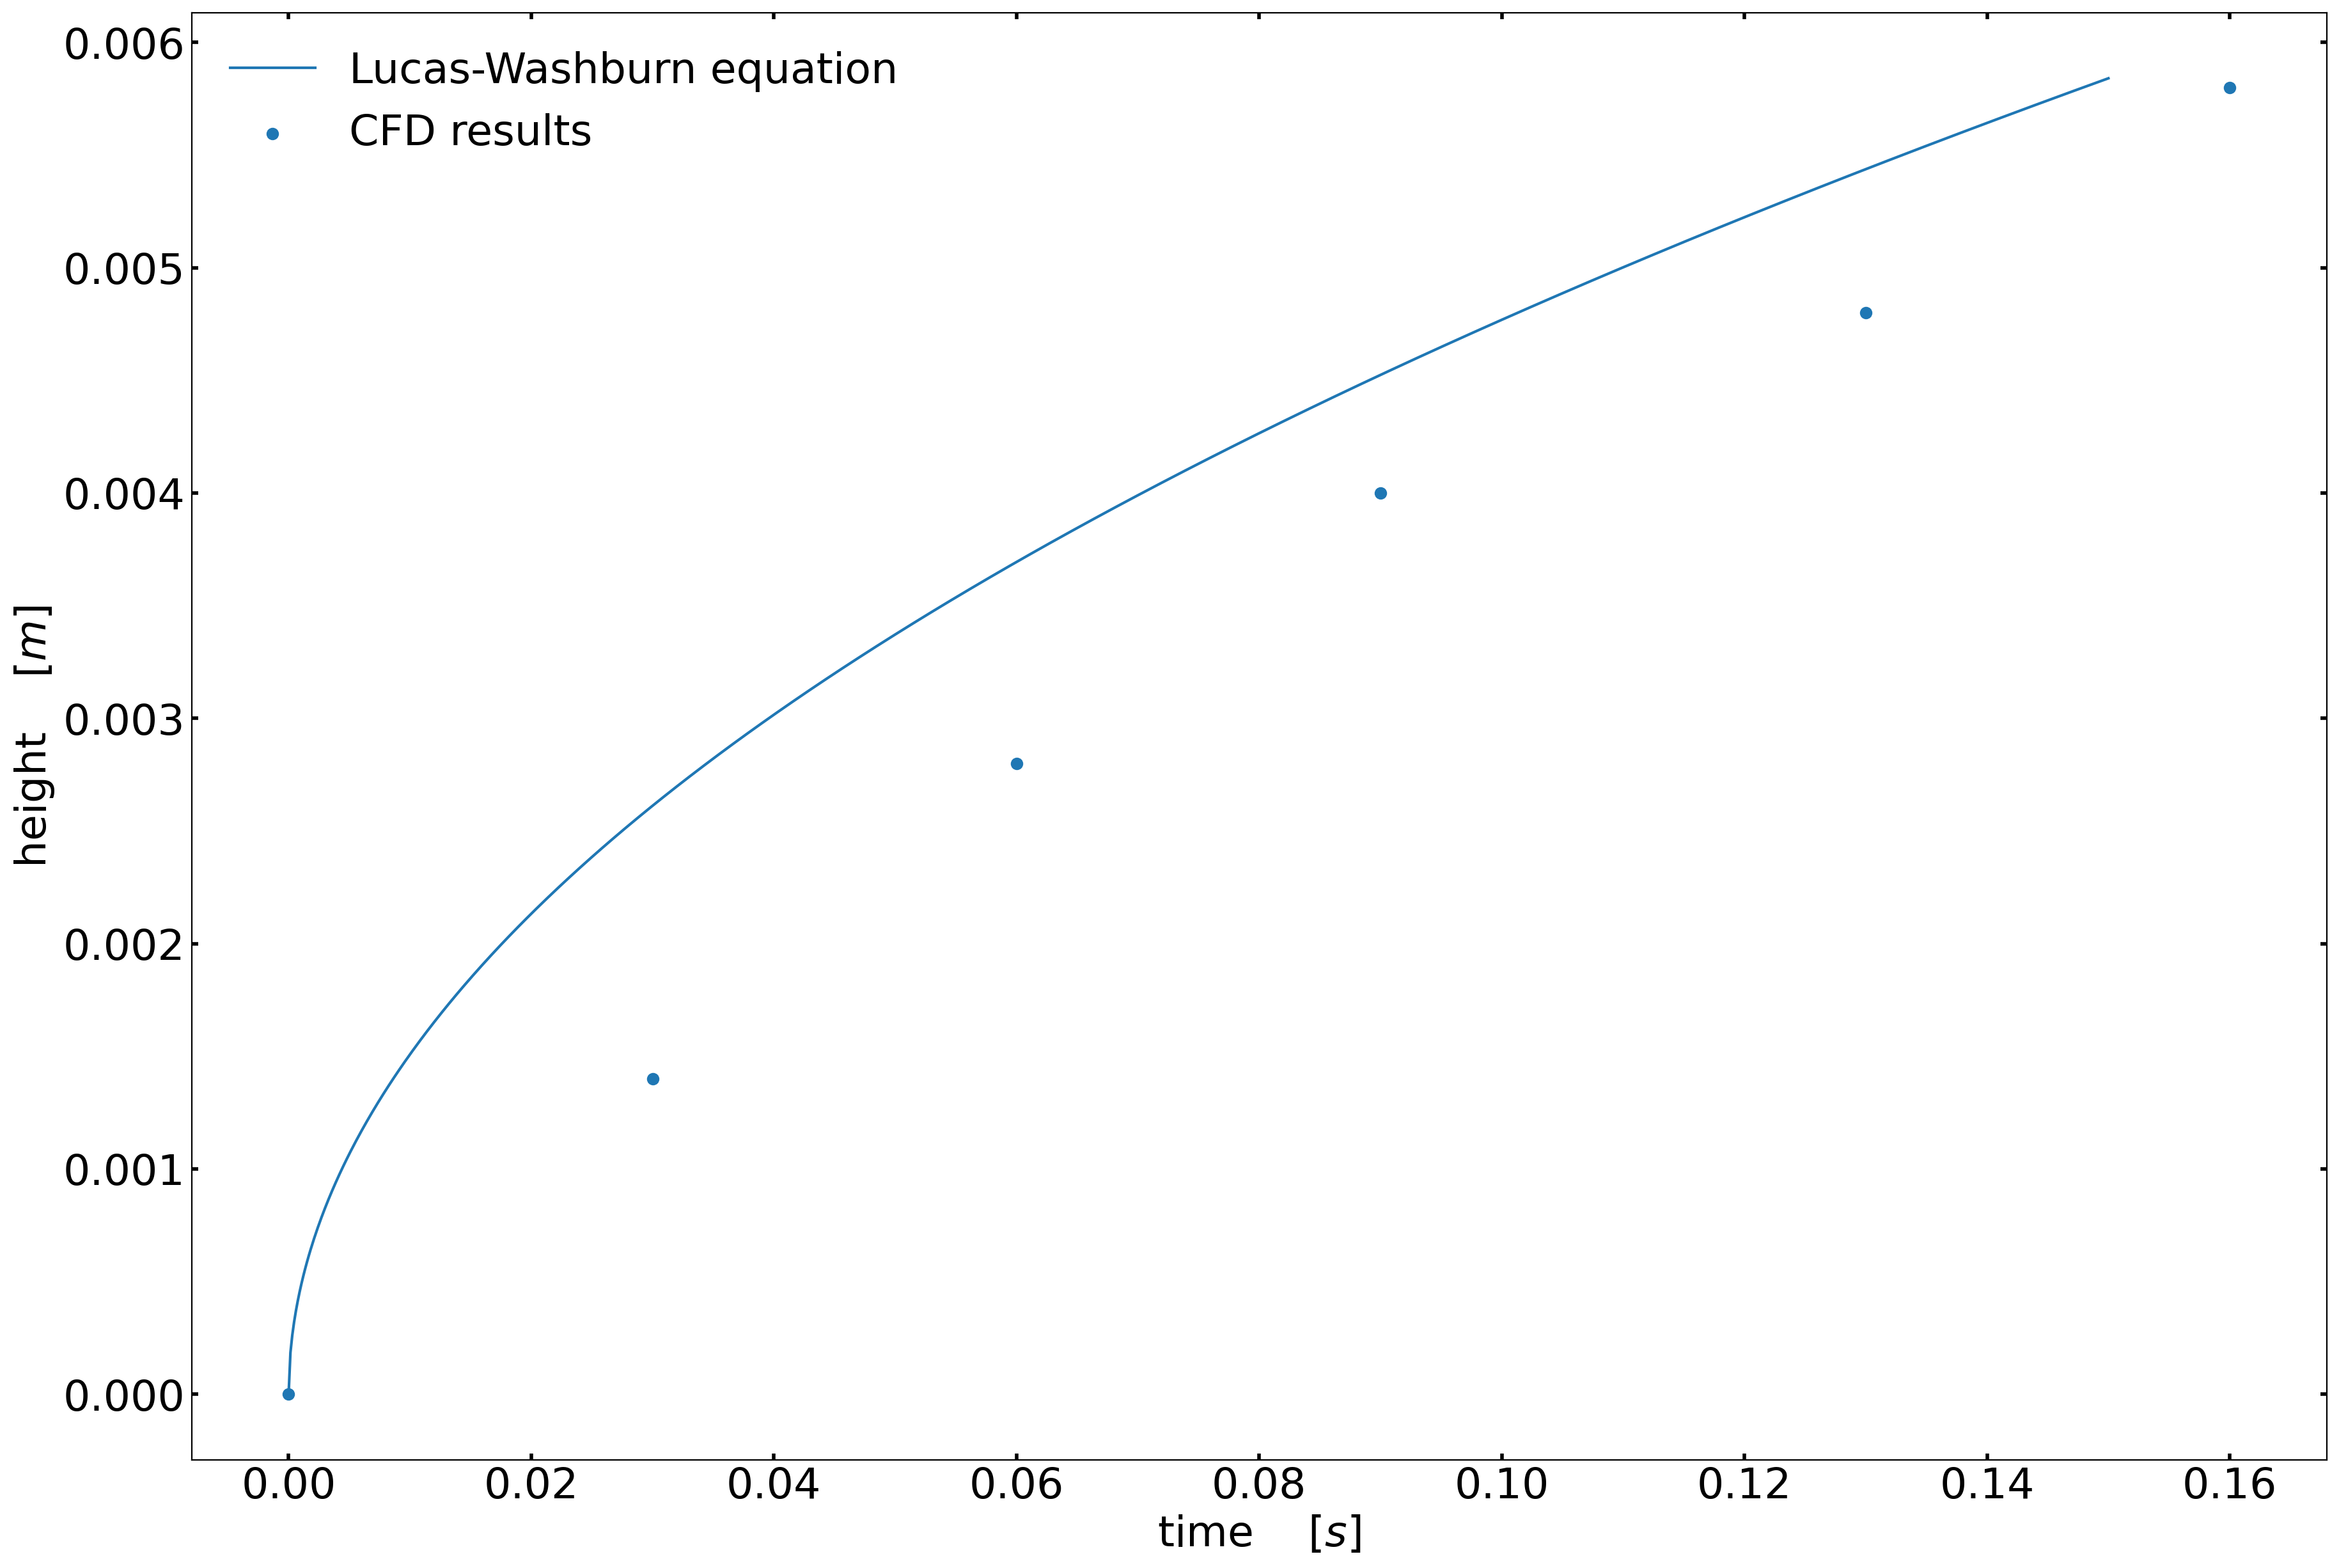
\includegraphics[width=1.00\textwidth]{./modelVScfd.png}
	\caption{CFD simulation results compared with Lucas–Washburn model predictions}
	\label{img:modelVScfd}
\end{figure}

in regards to the computational model, the mass and momentum equations can be written as: 

\begin{dmath}
\frac{\partial}{\partial t} (\rho \vec{v}) + \nabla \cdot (\rho \vec{v} \vec{v}) = - \nabla p + \nabla \cdot [\mu (\nabla \vec{v} + \nabla {\vec{v}}^t)] + \rho \vec{g}
\end{dmath}

\begin{dmath}
\frac{\partial \rho}{\partial t} + \nabla \cdot (\rho \vec{v}) = 0
\end{dmath}

with time $t$, density $\rho$, dynamic viscosity $\mu$, velocity vector $\vec{v}$, pressure $p$, and gravity $\vec{g}$. The Eulerian model was implemented to record the water-air interface in the capillary tube and in the water reservoir. The fluid heights (marked by the Eulerian interface) were measured at six different times using AmpScope software to compute the pixel-to-metric relationship using the model dimensions as a reference.

%\begin{dmath}
%\left( \begin{matrix}
%\textrm{Heat in}\\
%\textrm{via}\\
%\textrm{Convection}
%\end{matrix} \right) +
%\left( \begin{matrix}
%\textrm{Heat in}\\
%\textrm{via}\\
%\textrm{Radiation}
%\end{matrix} \right) = 0
%\end{dmath}

%\begin{figure}[h!]
%	\centering
%	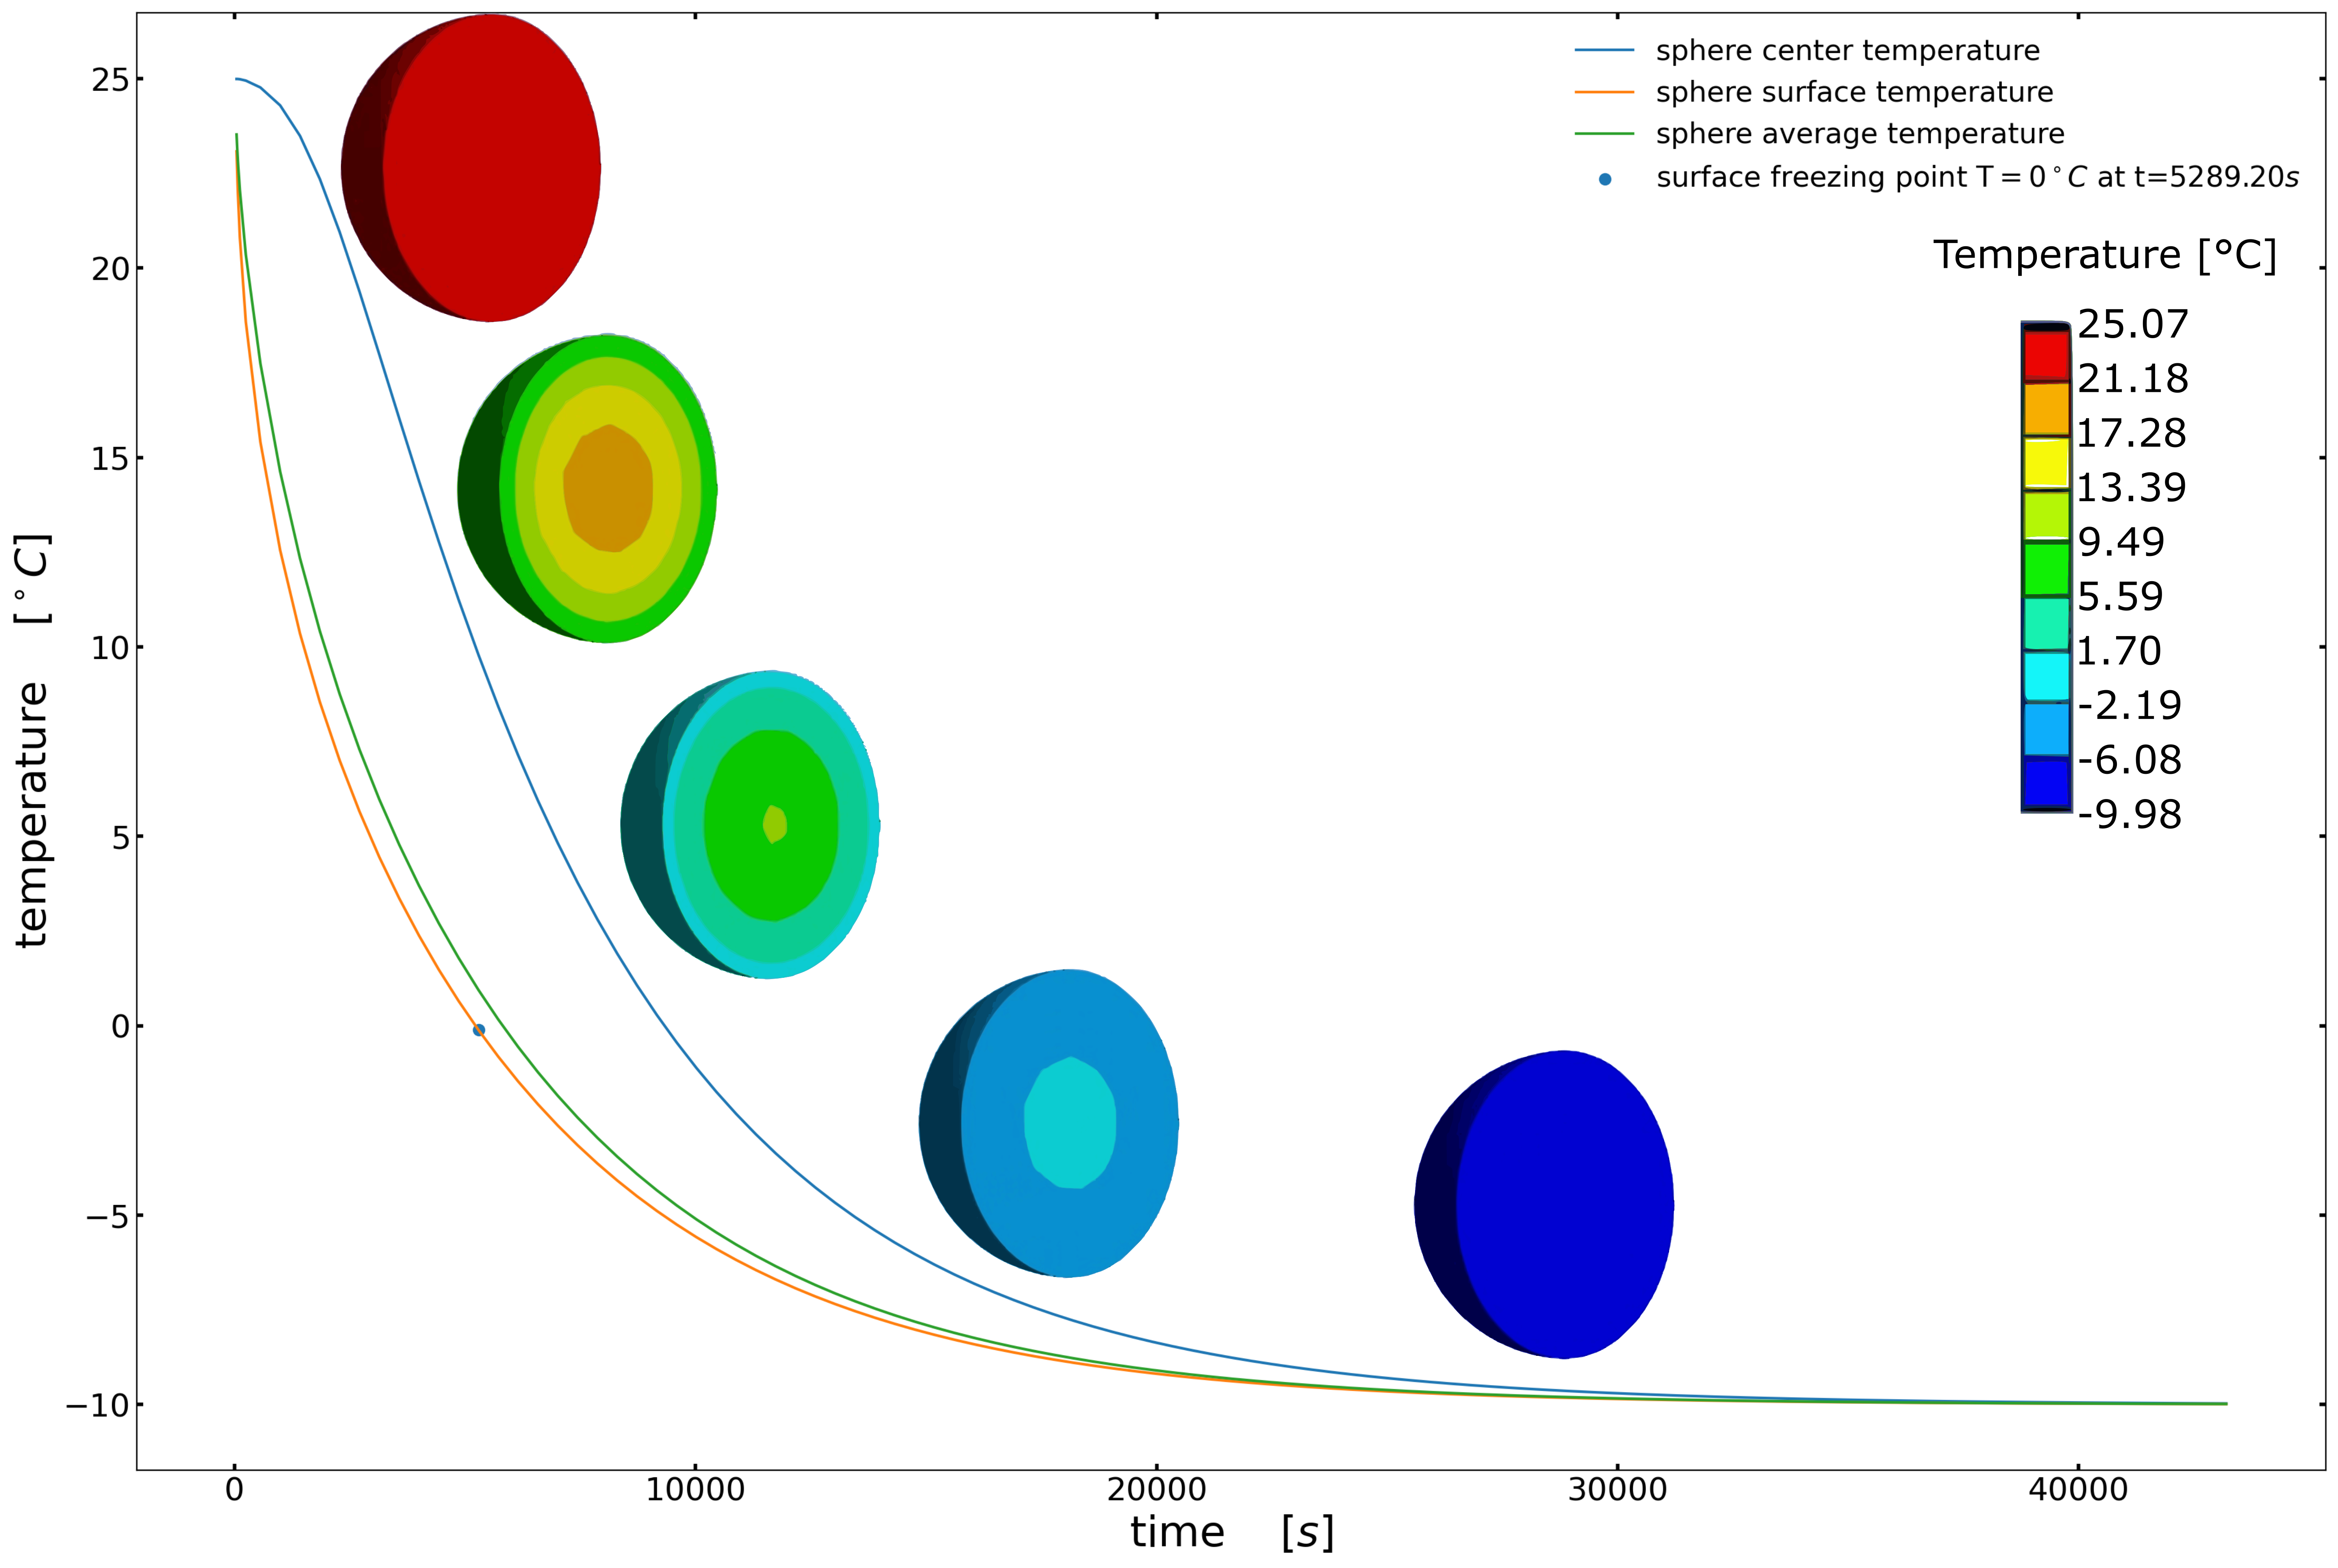
\includegraphics[width=1.00\textwidth]{./sphereTemps.png}
%	\caption{Visualization of a Velocity Field}
%	\label{img:sphereTemps}
%\end{figure}

\printbibliography[title={References}]
\end{document}
